\subsection{service}
\label{subsec:service}

\begin{figure}[H]
  \centering
  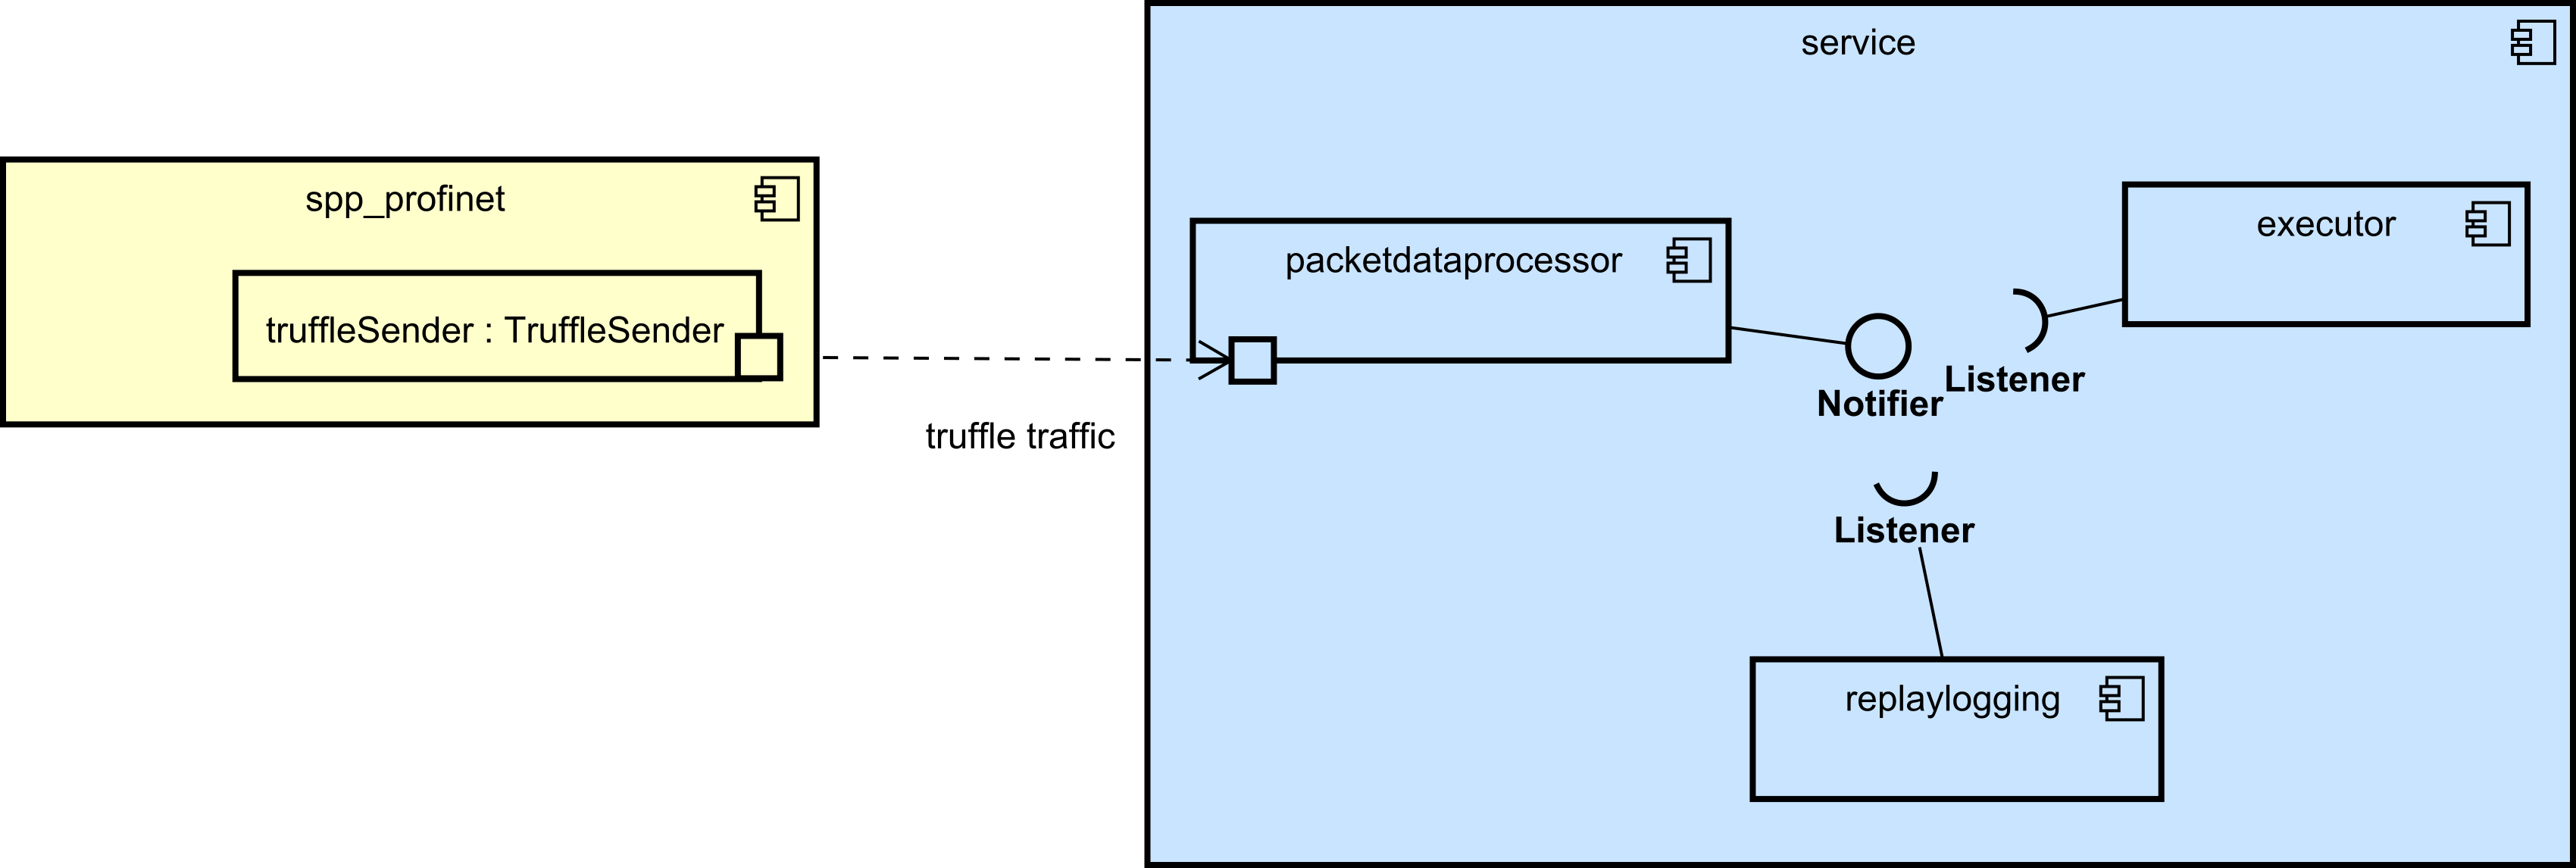
\includegraphics[width=\textwidth]{../diagramimages/service.png}
  \caption{service-Package}
\end{figure}

\medskip
Im service-Package befinden sich alle durchlaufenden Threads von \gls{programname},
mit Ausnahme vom \hyperref[subsec:view]{view}, das ein eigenes Package zur verzögerungsfreien Darstellung ist, und dem
main-Thread. Jedes Unterpackage kapselt dabei genau eine selbständig laufende Funktionalität, meist eine pro Thread. In den folgenden Abschnitten ist erklärt, was genau die Unterpackages packetdataprocessor, replaylogging und executor machen.

    \subsubsection{packetdataprocessor}
    \label{subsubsec:truffleprocessor}

    Der packetdataprocessor-Service läuft konstant im Hintergrund, in einem eigenen Thread,
    und empfängt die im \gls{sppname} erstellten Truffles.
    Diese packt er in ein Java-Truffle-Objekt, welches dann wiederum von dem
    \textit{TruffleReciever} in ein Command gesteckt wird. Da der \textit{TruffleReciever}
    auch ein \gls{notifier} ist, verschickt er den Command auch gleich an
    alle registrierten \gls{listener}, sodass der CommandExecutor die bekommt wo die Commands
    als nächstes auf dem Model angewandt werden.

    \clearpage
    \begin{sidewaysfigure}
      \centering
      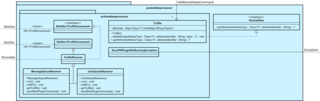
\includegraphics[width=\textwidth]{../diagramimages/packetdataprocessor.png}
      \caption{packetdataprocessor-Package}
    \end{sidewaysfigure}
    \clearpage

    \subsubsection{replaylogging}
    \label{subsubsec:replaylogging}

    Der replaylogging-Service besteht aus 2 Hauptaufgaben, die jeweils ihren eigenen Thread haben.
    Der erste ist der \textit{ReplayLogSaveService} und kümmert sich um das speichern das aktuellen
    Graphen. Der zweite ist der \textit{ReplayLogLoadService} und kümmert sich um das
    wiederherstellen eines gespeicherten Graphen.
    \newline
    \newline
    Der \textit{ReplayLogSaveService} läuft konstant im Hintergrund und empfängt alle
    vom \textit{TruffleReciever} verschickten Commands. Diese werden alle X
    Sekunden (vom Benutzter festlegbar) komprimiert und in eine Liste gepackt.
    Komprimiert heißt, dass viele Commands, die das selbe tun, in ein Command
    gepackt werden. Zusätzlich zu den Commands wird auch noch ein Snapshot
    von dem aktuellen Graphen gemacht, der dann zusammen mit der erstellten
    Command-Liste in ein ReplayLog-Objekt getan wird. Dieses
    ReplayLog-Objekt wird dann von Java serialisiert und gespeichert.
    \newline
    \newline
    Diese Logs können zu einem späteren Zeitpunkt wieder geladen werden um den
    Graphen wiederherzustellen. Dazu ist der \textit{ReplayLogLoadService} da. Wenn
    der User die Replayfunktion aktiviert, fängt der ReplayLogLoadService an die
    ReplayLogs zu laden. Dann wird in der view der Snapshotgraph angezeigt
    und die gespeicherten Commands aus dem ReplayLog werden auf
    diesem Snapshot angewandt. Der ReplayLogLoadService kontrolliert somit die
    Wiedergabe des alten Graphen und kann sogar hin und her zwischen Snapshots
    springen (momentan nicht zwischen einzelnen Commands, da dieses keine undo-
    und redo-Funktion besitzten).
    \newline
    \newline
    Der ReplayLogLoadService läuft in seinem eigenen Thread, weil er sich darum
    kümmert das immer genügend Daten im Speicher liegen. In anderen Worten, er
    buffert die Replaylogs vor damit sich der Graph bei dem Benutzter flüssig
    abspielt.

    \clearpage
    \begin{sidewaysfigure}
      \centering
      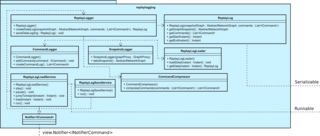
\includegraphics[width=\textwidth]{../diagramimages/replaylogging.png}
      \caption{replaylogging-Package}
    \end{sidewaysfigure}
    \clearpage

    \subsubsection{executor}
    \label{subsubsec:executor}

    \begin{figure}[H]
      \centering
      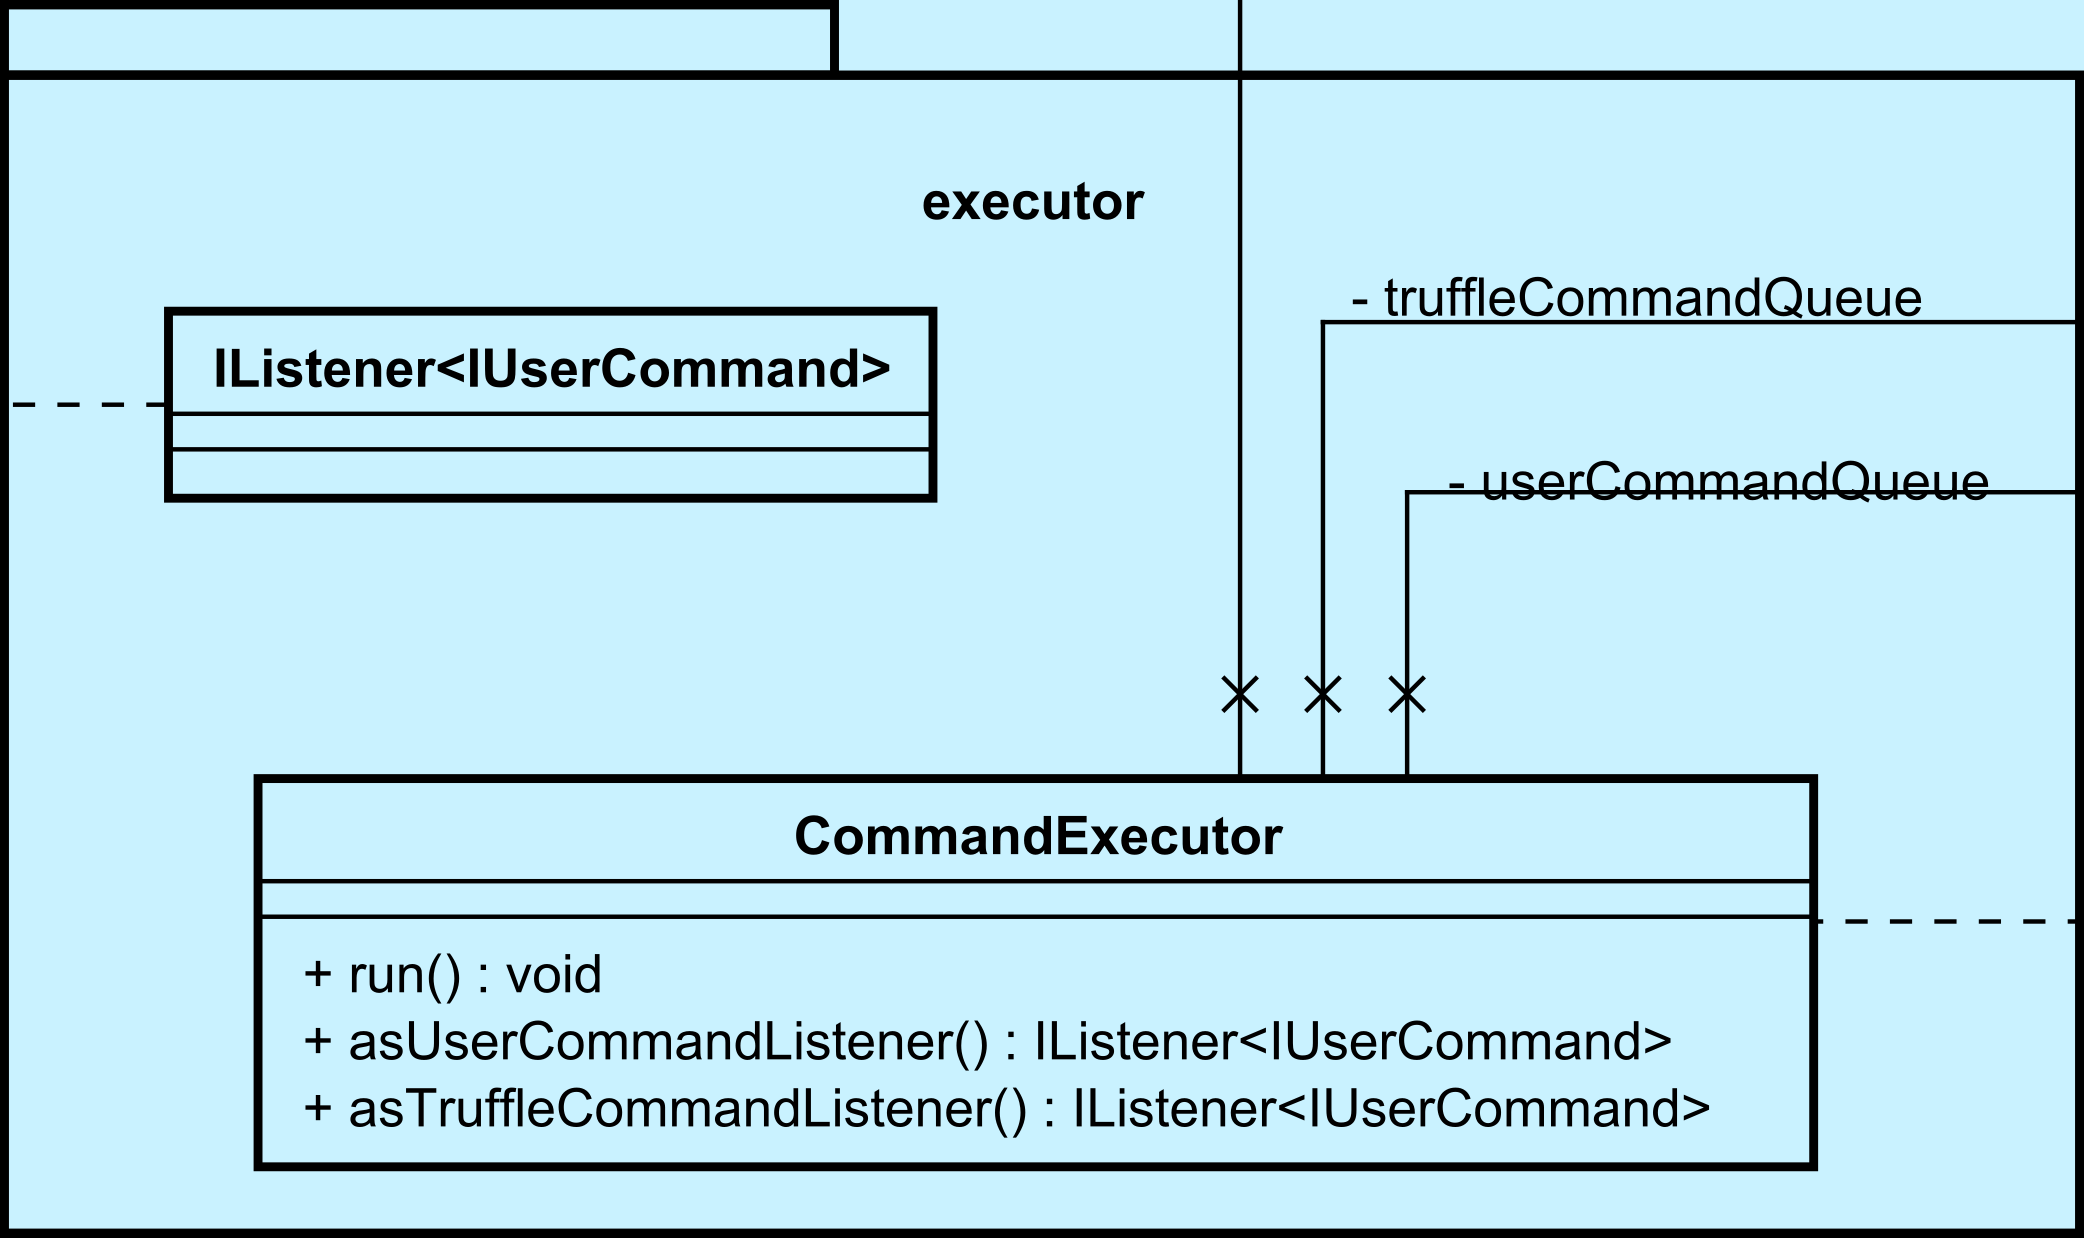
\includegraphics[width=\textwidth]{../diagramimages/executor.png}
      \caption{executor-Package}
    \end{figure}

    \medskip
    Der executor-Service läuft auch wieder konstant im Hintegrund in seinem
    eigenen Thread. Er ist ein \gls{listener} der sowohl bei dem TruffleReciever aus dem
    \hyperref[subsubsec:packetdataprocessor]{packetdataprocessor}-Package als
    auch bei den view-Controllern aus dem \hyperref[subsec:view]{view}-Package
    registriert ist. D.h. er bekommt, wie das \hyperref[subsubsec:replaylogging]{replaylogging},
    alle \hyperref[subsubsec:trufflecommand]{TruffleCommands} und führt diese
    dann auf dem aktuellen Model aus.
    \newline
    \newline
    In \gls{programname} gibt es zwei Instanzen vom Executor. Die erste bearbeitet
    den aktuellen Graphen und die zweite bearbeitet die Snapshot-Instanz, falls
    eine existiert. So kann der aktuelle Graph auf dem neusten Stand bleiben, während
    gleichzeitig der Benutzter einen alten Graphen aus
    ReplayLogs rekonstruiert anschaut.